\section{List of model features/parameters and their biological foundation}
\section{Visual closeness}
\subsection{Ventral Furrow}
After mitosis stops, the the first visual change on the is the belly, where a distinct cleft begins forming. \\

The cells do not constrict indiscriminately, instead starting with the \textit{inner} 8x60 cells. As the furrow closes off, creating closed-off tube with a recognizable light bulb-shape in the cross section, the inaginated tissue "disconnects".

\begin{figure}[H]
    \centering
    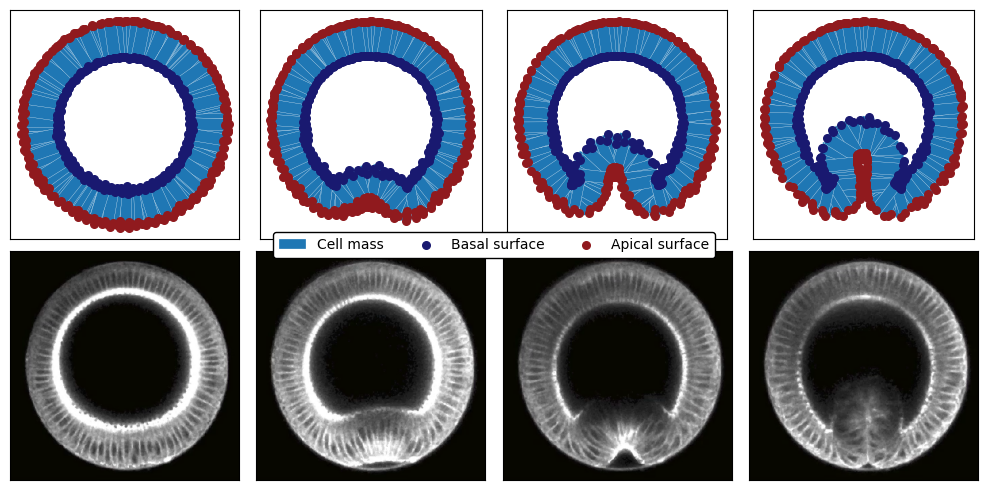
\includegraphics[width=0.7\linewidth]{chapters/Results/figures/VF_comparison.png}
    \caption{A comparison of simulation and frames from live develiopment. Cross section video is taken from \cite{}}
    \label{fig:enter-label}
\end{figure}
\subsection{Germ band}
\subsection{Auxiliary furrows}
\subsection{Daniel}
\section{Quantitative closeness}
\subsection{Movements}
\subsection{Timing}
\subsection{Strain}
\subsection{Rosettes}
\subsection{Daniel-data?}
\newpage
\section{In Silico Mutant "predictions" - compared to phenotypes and reference model}
\subsection{No PMG}
% Twist and shout
\subsection{No Ventral Furrow}
% \url{https://genesdev.cshlp.org/content/5/9/1568.full.pdf}
% We are seeing the right thing
\subsection{No Cephalic Furrow?}
% maybe not important
\subsection{No active intercolation / Germ band}
% \url{https://softmath.seas.harvard.edu/wp-content/uploads/2019/10/2009-07.pdf}
% clear that model is missing cell shape change!
\section{Additive/subtractive working together matrix}
% \subsubsection{}